\documentclass[tikz, border=12pt]{standalone}
\usepackage{tikz}
\usetikzlibrary{arrows.meta, positioning}

\definecolor{commander}{HTML}{1B2A4A}
\definecolor{agent}{HTML}{3B5BA9}
\definecolor{tool}{HTML}{1C8C7C}
\definecolor{lifeline}{HTML}{9CA3AF}
\definecolor{edge}{HTML}{3F3F46}
\definecolor{activ}{HTML}{E8EAF0}
\definecolor{selfmsg}{HTML}{1C8C7C}

\begin{document}
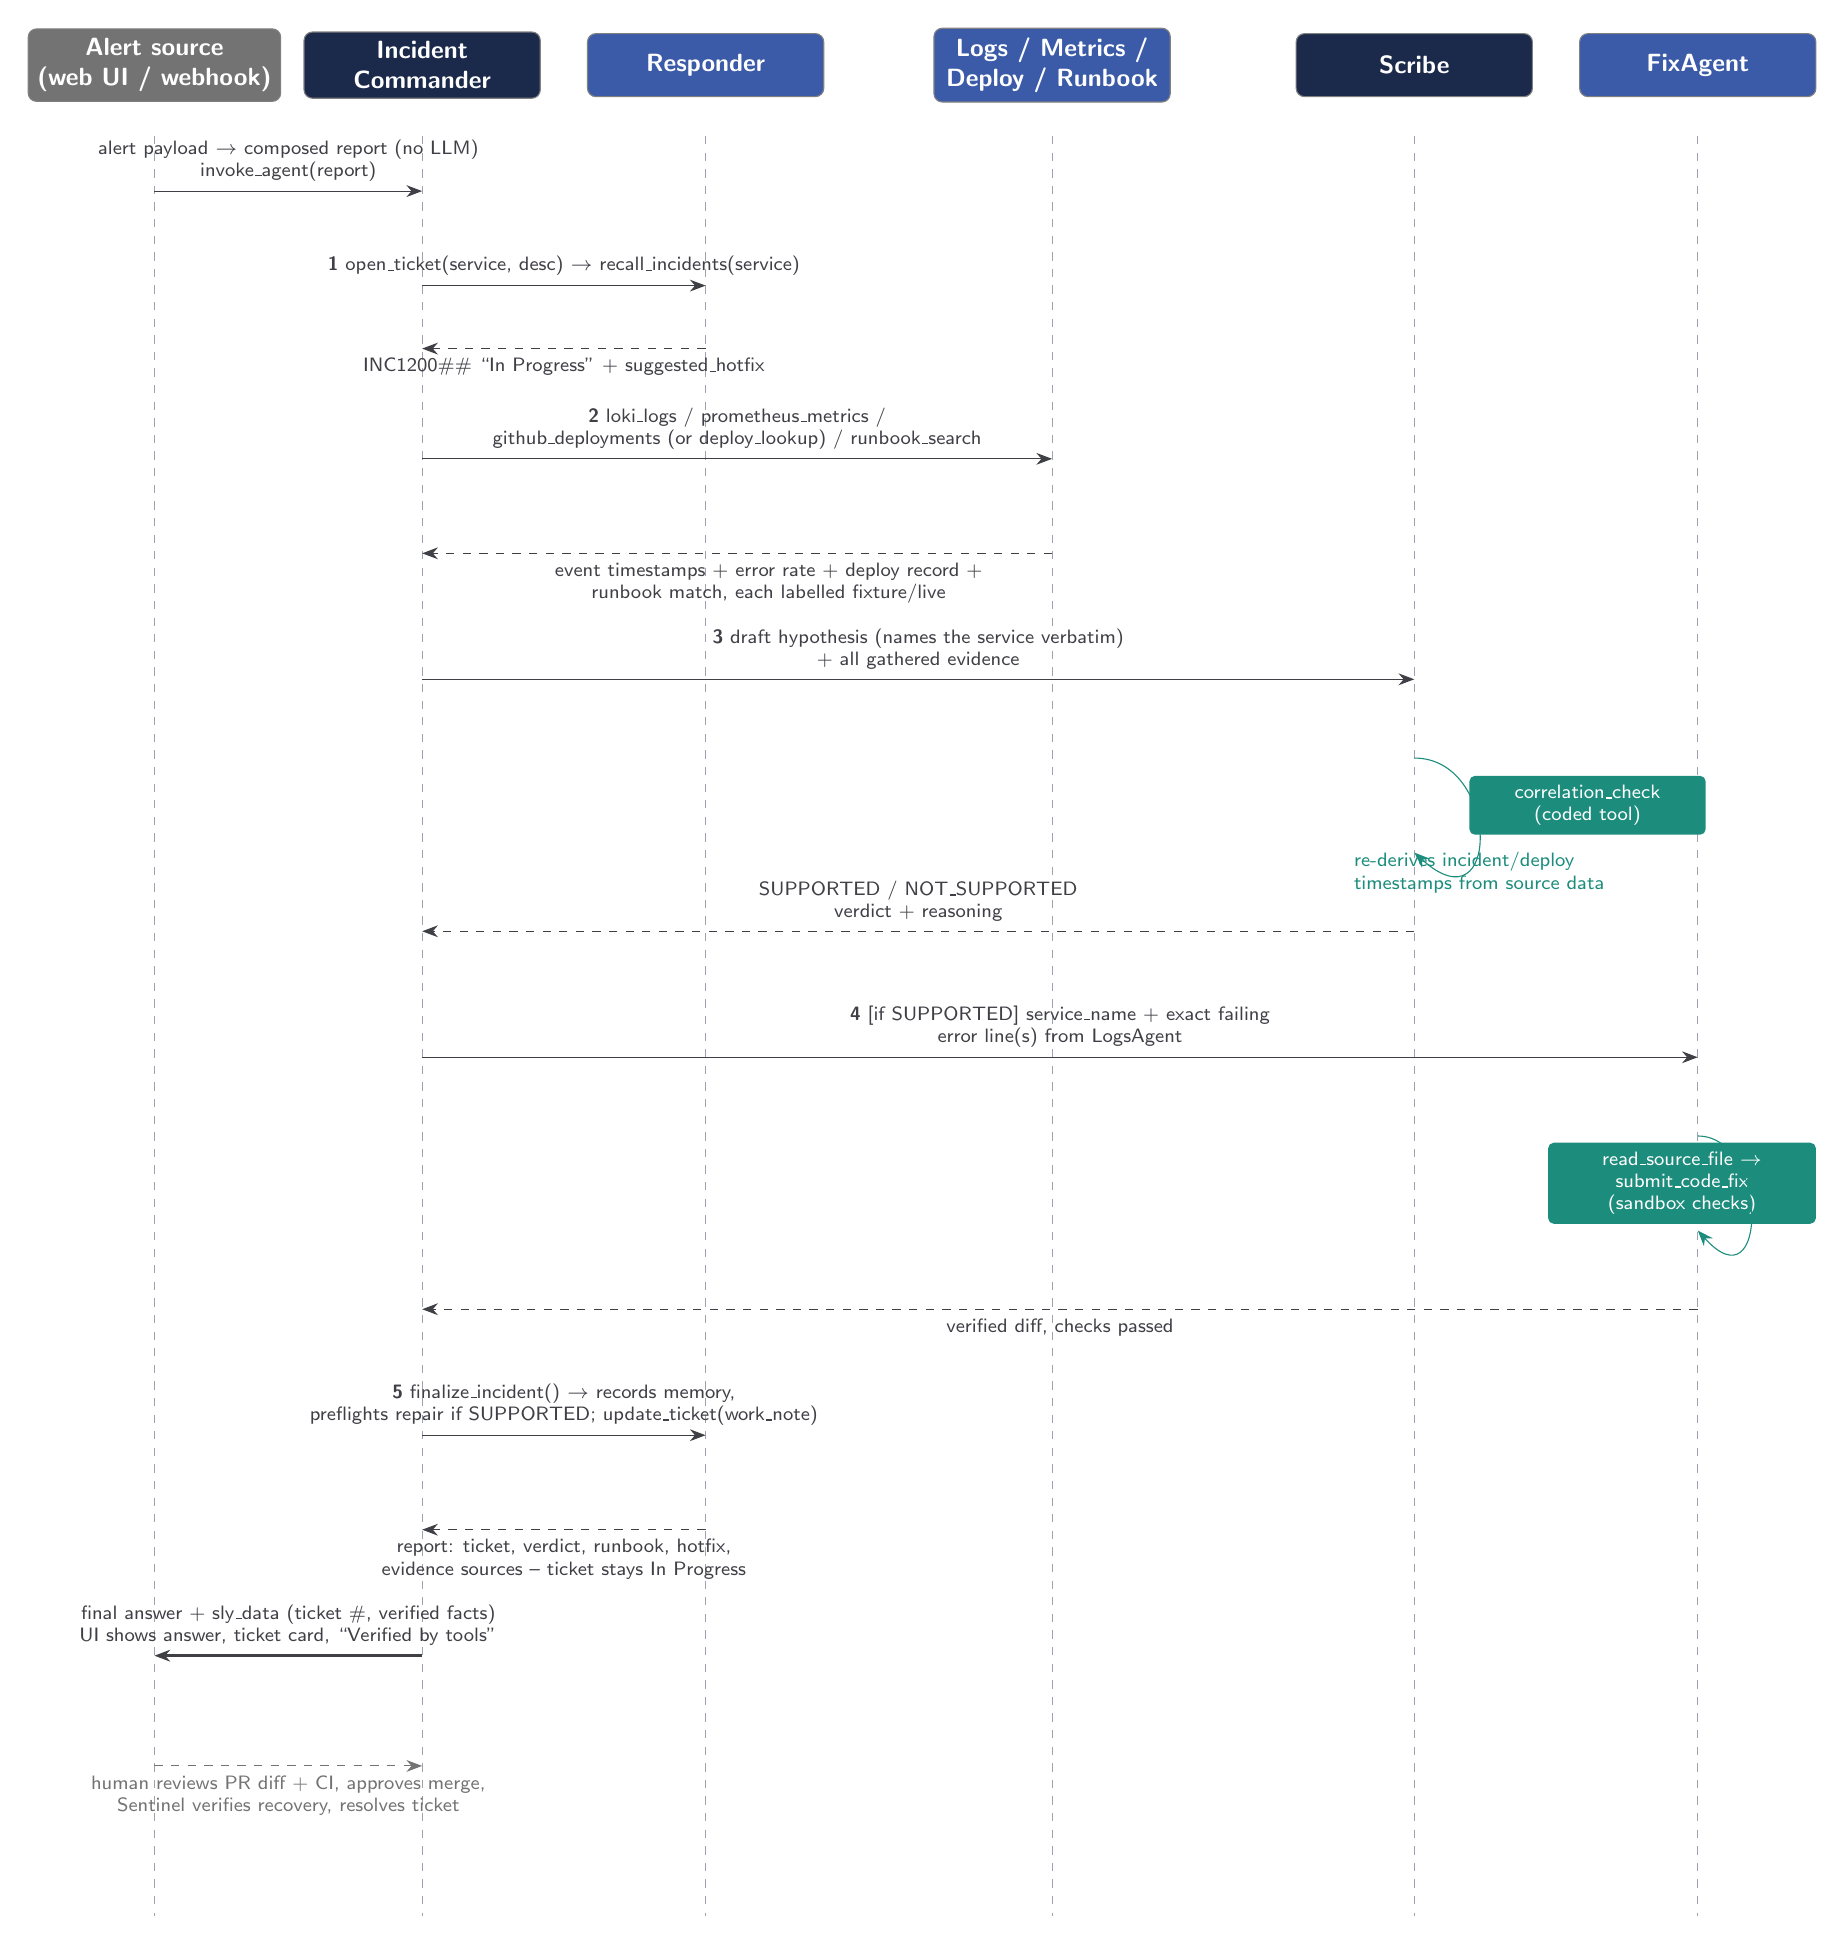
\begin{tikzpicture}[
  font=\sffamily,
  >=Stealth,
  >={Stealth[length=2.2mm]},
  every node/.style={align=center},
  actor/.style={rounded corners=3pt, draw=black!50, fill=#1, text=white, font=\sffamily\small\bfseries, minimum width=30mm, minimum height=8mm},
  msg/.style={-{Stealth[length=2mm]}, color=edge, font=\sffamily\scriptsize},
  ret/.style={-{Stealth[length=2mm]}, color=edge, dashed, font=\sffamily\scriptsize},
  lifel/.style={color=lifeline, dashed},
  actv/.style={fill=activ, draw=black!30},
]

% ---- x-coordinates for each lifeline ----
\def\xA{0}     % Alert Source
\def\xC{3.4}   % IncidentCommander
\def\xR{7.0}   % Responder
\def\xS{11.4}  % Evidence specialists (Logs/Metrics/Deploy/Runbook)
\def\xSc{16.0} % Scribe
\def\xF{19.6}  % FixAgent

\def\ytop{0}

% ---- Actor headers ----
\node[actor=black!55] (A) at (\xA,\ytop) {Alert source\\(web UI / webhook)};
\node[actor=commander] (C) at (\xC,\ytop) {Incident\\Commander};
\node[actor=agent] (R) at (\xR,\ytop) {Responder};
\node[actor=agent] (S) at (\xS,\ytop) {Logs / Metrics /\\Deploy / Runbook};
\node[actor=commander] (Sc) at (\xSc,\ytop) {Scribe};
\node[actor=agent] (F) at (\xF,\ytop) {FixAgent};

% ---- lifelines ----
\def\ybot{-23.5}
\foreach \x in {\xA,\xC,\xR,\xS,\xSc,\xF} {
  \draw[lifel] (\x,-0.9) -- (\x,\ybot);
}

% 0. Alert -> Commander
\draw[msg] (\xA,-1.6) -- node[above, pos=0.5, align=center]{alert payload $\rightarrow$ composed report (no LLM)\\invoke\_agent(report)} (\xC,-1.6);

% 1. Commander -> Responder (open ticket + recall)
\draw[msg] (\xC,-2.8) -- node[above, pos=0.5]{\textbf{1} open\_ticket(service, desc) $\rightarrow$ recall\_incidents(service)} (\xR,-2.8);
\draw[ret] (\xR,-3.6) -- node[below, pos=0.5]{INC1200\#\# ``In Progress'' + suggested\_hotfix} (\xC,-3.6);

% 2. Commander -> Specialists (parallel fan-out, all four required)
\draw[msg] (\xC,-5.0) -- node[above, pos=0.5, align=center]{\textbf{2} loki\_logs / prometheus\_metrics /\\github\_deployments (or deploy\_lookup) / runbook\_search} (\xS,-5.0);
\draw[ret] (\xS,-6.2) -- node[below, pos=0.45, align=center]{event timestamps + error rate + deploy record +\\runbook match, each labelled fixture/live} (\xC,-6.2);

% 3. Commander -> Scribe
\draw[msg] (\xC,-7.8) -- node[above, pos=0.5, align=center]{\textbf{3} draft hypothesis (names the service verbatim)\\+ all gathered evidence} (\xSc,-7.8);

% 3'. Scribe self-call: correlation_check
\node[rounded corners=2pt, fill=tool, text=white, font=\sffamily\scriptsize, minimum width=30mm, minimum height=7mm] at (\xSc+2.2,-9.4) {correlation\_check\\(coded tool)};
\draw[msg, color=selfmsg] (\xSc,-8.8) .. controls +(1.1,0) and +(1.1,-1.0) .. node[below=1mm, align=left, text=selfmsg, font=\sffamily\scriptsize]{re-derives incident/deploy\\timestamps from source data} (\xSc,-10.0);

% 3''. Scribe -> Commander
\draw[ret] (\xSc,-11.0) -- node[above, pos=0.5, align=center]{SUPPORTED / NOT\_SUPPORTED\\verdict + reasoning} (\xC,-11.0);

% 4. Commander -> FixAgent (only if SUPPORTED)
\draw[msg] (\xC,-12.6) -- node[above, pos=0.5, align=center]{\textbf{4} [if SUPPORTED] service\_name + exact failing\\error line(s) from LogsAgent} (\xF,-12.6);
\node[rounded corners=2pt, fill=tool, text=white, font=\sffamily\scriptsize, minimum width=34mm, minimum height=7mm] at (\xF-0.2,-14.2) {read\_source\_file $\rightarrow$\\submit\_code\_fix\\(sandbox checks)};
\draw[msg, color=selfmsg] (\xF,-13.6) .. controls +(0.9,0) and +(0.9,-1.0) .. (\xF,-14.8);
\draw[ret] (\xF,-15.8) -- node[below, pos=0.5, align=center]{verified diff, checks passed} (\xC,-15.8);

% 5. Commander -> Responder (finalize + update/resolve)
\draw[msg] (\xC,-17.4) -- node[above, pos=0.5, align=center]{\textbf{5} finalize\_incident() $\rightarrow$ records memory,\\preflights repair if SUPPORTED; update\_ticket(work\_note)} (\xR,-17.4);
\draw[ret] (\xR,-18.6) -- node[below, pos=0.5, align=center]{report: ticket, verdict, runbook, hotfix,\\evidence sources -- ticket stays In Progress} (\xC,-18.6);

% 6. Commander -> Alert source (final answer)
\draw[msg, line width=0.9pt] (\xC,-20.2) -- node[above, pos=0.5, align=center]{final answer + sly\_data (ticket \#, verified facts)\\UI shows answer, ticket card, ``Verified by tools''} (\xA,-20.2);

% 7. Human review (outside the agent network)
\draw[ret, color=black!55] (\xA,-21.6) -- node[below, pos=0.5, align=center]{\scriptsize human reviews PR diff + CI, approves merge,\\\scriptsize Sentinel verifies recovery, resolves ticket} (\xC,-21.6);

\end{tikzpicture}
\end{document}
